\documentclass[a4paper,titlepage,12pt]{article}
\usepackage[utf8]{inputenc}
\usepackage[T1]{fontenc}
\usepackage[magyar]{babel}
\usepackage{graphicx}
\usepackage{float}
\usepackage{grffile}
\usepackage{amssymb}
\setlength\parindent{0pt}
\begin{document}

	\begin{centering}
		\scshape\LARGE Folytonos közegek mechanikája (emelt szint) \par
		\vspace{1cm}
		
		\large 8. tétel: Ideális folyadék áramlása, Bernoulli törvény és alkalmazása
	\end{centering}

\part*{Ideális folyadék}

Az ideális folyadék felveszi a tárolásra szolgáló edény alakját, megtartja a térfogatát, gyakorlatilag összenyomhatatlan. 

Áramlás során 3 fő mennyiségünk van: $$\varrho(\underline{r},t)$$ $$p(\underline{r},t)$$ $$\underline{v}(\underline{r},t) $$

\vspace{0.25 cm}
Az anyagmegmaradás miatt egy felületen beáramló anyag meg kell hogy egyezzen a felületen belül lévő anyag koncentrációjának a megváltozásával: $$ \frac{d}{dt}\int\varrho(r,t)dV+\oint\varrho \underline{v}d\underline{A}=0 $$

A Gauss-tétel felhasználásával a kontinuitási egyenletre az alábbi képletet kapjuk: $$\frac{d\varrho}{dt}+div(\varrho\underline{v})=0 $$

Stacionárius áramlás esetén $\varrho , v$ és $p$ időben állandól, ekkor $div(\varrho\underline{v})=0$. (Ebből viszont még nem következik, hogy a folyadék összenyomhatatlan.)

\vspace{0.25 cm}
Bevezethetjük az áramlási vonalakat. Ez egy olyan vektortér, amely a tér minden pontjához hozzárendeli az ottani sebességvektort. Az áramvonalak érintői minden pontban megegyeznek a sebesség irányával. Az áramvonalak sűrűsége jelzi a sebességet. 

\begin{figure}[H]
	\begin{center}
		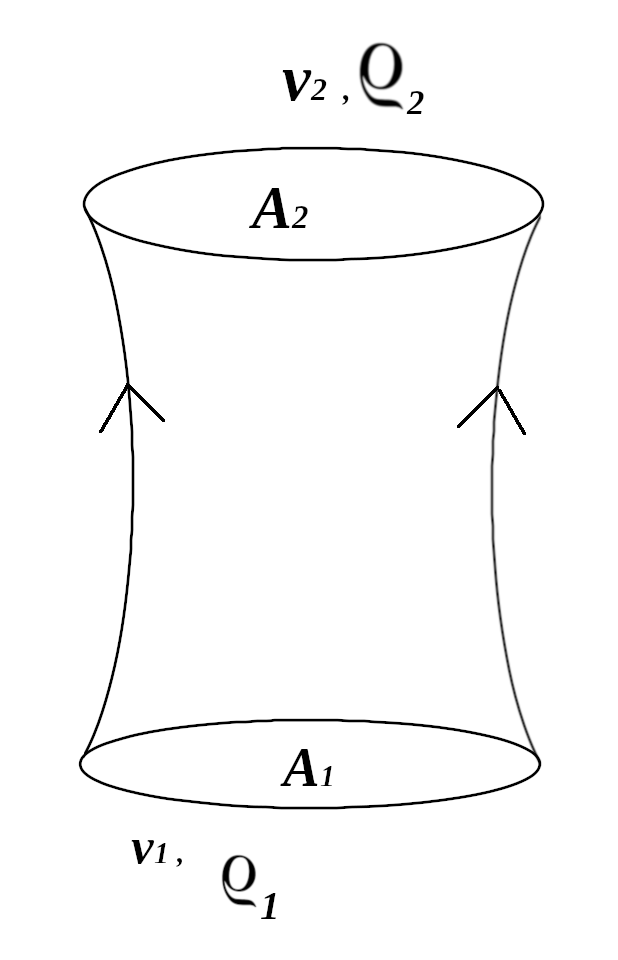
\includegraphics[width=0.3\textwidth]{tetel8.png}
		\caption{Az áramlási tér. A két végén $\varrho vA=const.$}
	\end{center}
\end{figure}

A folyadék térfogata nem változhat, $\varrho_{1}v_{1}A_{1}=\varrho_{2}v_{2}A_{2}$. Ha a folyadék összenyomhatatlan, $vA=$áll. Erre példa a csapaból kifolyó víz. Ahol nagyobb a sebessége, ott a kersztmetszete kisebb. 

A mozgásegyenlet szilárd testek esetén: $\varrho\underline{\ddot{u}}=\underline{f}+div\hat{\sigma}$. Mivel folyadékoknál $\underline{u}$-t nem definiáltuk, de $\ddot{u}=\frac{d}{dt}v(\underline{r}(t),t) $

\vspace{0.25 cm}
Az úgynevezett anyagi derivált: $$a_{i}=\frac{\partial v_{i}}{\partial t}+\frac{\partial v_{i}}{\partial x}\frac{\partial x}{\partial t}+\frac{\partial v_{i}}{\partial y}\frac{\partial y}{\partial t}+\frac{\partial v_{i}}{\partial z}\frac{\partial z}{\partial t} $$ $$\underline{a}=(\underline{v}\hspace{0.1 cm}\underline{\triangledown})\underline{v}+\frac{\partial v}{\partial t}$$

Ezt a mozgásegyenletbe behelyettesítve : $$\varrho[(\underline{v}\hspace{0.1 cm}\underline{\triangledown})\underline{v}+\frac{\partial v}{\partial t}]=\underline{f}+div\hat{\sigma}$$

Ideális folyadék esetén $\hat{\sigma}=-p\hat{I}$ (nincs belső surlódás, viszkozitás). Így $div\hat{\sigma}=-grad\hspace{0.05 cm}p$. Így ideális folyadékokra, stacionárius áramlás esetén $$\varrho[(\underline{v}\hspace{0.1 cm}\underline{\triangledown})\underline{v}]=\underline{f}-grad\hspace{0.05 cm}p $$

Az áramlási csövet vizsgálva $$\Delta m=\varrho_{1}v_{1}A_{1}\Delta t=\varrho_{2}v_{2}A_{2}\Delta t $$ tömegű folyadék áramlik át $\Delta t$ idő alatt.

A munkatétel alapján: $$\frac{1}{2}\Delta mv_{2}^{2}-\frac{1}{2}\Delta mv_{1}^{2}=p_{1}v_{1}A_{1}\Delta t-p_{2}v_{2}A_{2}\Delta t+\Delta m U_{1}-\Delta m U_{2}+\Delta\delta W$$

A helyzeti energia $\delta W$ a belső erők munkája. Összenyomhatatlan folyadék esetén $\Delta\delta W=0$  .

$$\frac{1}{2}v_{2}^{2}-\frac{1}{2}v_{1}^{2}=\frac{p_{1}A_{1}v_{1}\Delta t}{A_{1}\varrho_{1}v_{1}\Delta t}-\frac{p_{2}A_{2}v_{2}\Delta t}{A_{2}\varrho_{2}v_{2}\Delta t}+U_{1}-U_{2} $$

Ezt az egyenletet egyszerűsítve a következő alakot kapjuk: $$\frac{1}{2}v_{2}^{2}-\frac{1}{2}v_{1}^{2}=\frac{p_{1}}{\varrho_{1}}-\frac{p_{2}}{\varrho_{2}}+U_{1}-U_{2} $$

\part*{Bernoulli törvény}

Az előző egyenletben adott indexeket egy oldalra rendezve látszik, hogy: $$\frac{1}{2}v^{2}+\frac{p}{\varrho}+U=const.$$

Ezt nevezzük Bernoulli törvénynek. Ez mozgó felületekre nem alkalmazható!

Gáz esetén a Bernoulli-tövény: $$dU_{k}=\delta Q+\delta W_{k}$$ $$dU_{b}=\delta Q-\delta W_{b} $$

Feltételezzük, hogy a folyamat adiabatikus, azaz $\delta W_{k}=-dU_{b}=-C_{V}m \cdot dT$

$$\frac{p}{\varrho}=\frac{R}{M}T\longrightarrow T=\frac{P}{\varrho}\frac{M}{R}$$
$$ C_{p}-C_{V}=\frac{R}{M} $$  $$\frac{C_{p}}{C_{V}}-1=\frac{1}{C_{V}}\frac{R}{M} $$ $$C_{V}T=C_{V}\frac{M}{R}\frac{p}{\varrho} $$ $$ C_{V}T=\frac{1}{\frac{C_{p}}{C_{V}}-1}\frac{p}{\varrho} $$ $$\frac{1}{2}v_{2}^{2}+\frac{p_{2}}{\varrho_{2}}+\frac{1}{\kappa-1}\frac{p_{2}}{\varrho_{2}}=\frac{1}{2}v_{1}^{2}+\frac{p_{1}}{\varrho_{1}}+\frac{1}{\kappa-1}\frac{p_{1}}{\varrho_{1}} $$

Így is megkaptuk a Bernoulli-törvényt a következő alakban: $$\frac{1}{2}v^{2}+\frac{\kappa}{\kappa-1}\frac{p}{\varrho}+U=const. $$

\part*{Változó keresztmetszetű csőben áramló gáz}

Az anyagmegmaradás alapján: $\varrho vA=$áll.

Adiabatikus közelítés: $pv^{\kappa}=$áll. , $\frac{p}{\varrho^{\kappa}}=$áll.

$$d(\varrho vA)=vAd\varrho+\varrho AdV+\varrho vdA=0 $$
$$\frac{d\varrho}{\varrho}+\frac{dv}{v}+\frac{dA}{A}=0 $$

Felhasználva, a Bernoulli ideális gázra kapott egyenletét: $$d(\frac{v^{2}}{2}+\frac{\kappa}{\kappa-1}\frac{p}{\varrho})=vdv+\frac{\kappa}{\kappa-1}(\frac{dp}{\varrho}-\frac{p}{\varrho^{2}}d\varrho)=0 $$

Mivel a nyomás függ a sűrűségtől: $$dp(\varrho)=\frac{dp}{d\varrho}=c^{2}d\varrho$$

Itt $c^{2}=\frac{dp}{d\varrho}$, sebességnégyzet dimenziójú, $c$ pedig a hangsebesség. $$dv(v)+\frac{\kappa}{\kappa-1}(c^{2}\frac{d\varrho}{\varrho}-\frac{p}{\varrho}\frac{d\varrho}{\varrho})=0$$

Hogyha ismerjük, hogy $p=$áll., azaz $\frac{p}{\varrho^{\kappa}}=$áll. Ebből következően: $$\frac{dp}{d\varrho}=\frac{d}{d\varrho}(const.\cdot\varrho)=const.\cdot\kappa\varrho^{\kappa-1}=\frac{p}{\varrho^{\kappa}}\kappa\varrho^{\kappa-1}=\kappa\frac{p}{\varrho}=c^{2}\longrightarrow\frac{c^{2}}{\kappa}=\frac{p}{\varrho}$$

Ezt ismerve az egyenletünk új alakja: $$dv(v)+\frac{\kappa}{\kappa-1}(c^{2}-\frac{c^{2}}{\kappa})\frac{d\varrho}{\varrho}=0$$

Ez leegyszerűsödik arra, hogy:

$$dv(v)+c^{2}\frac{d\varrho}{\varrho}=0$$

És ha ezt rendezzük, akkor előáll, hogy: $$\frac{d\varrho}{\varrho}=
-\frac{v}{c^{2}}dv=-\frac{dv}{v}-\frac{dA}{A}$$ $$\frac{v^{2}}{c^{2}}\frac{dv}{v}-\frac{dv}{v}=\frac{dA}{A} $$ $$\frac{dA}{A}=(\frac{v^{2}}{c^{2}}-1)\frac{dv}{v} $$

Az utolsó egyenletből megfigyelhetjük, hogyha v<c, akkor a keresztmetszet csökkentésével a közeg sebességével nő.

Ha v>c, akkor a közeg sebessége a keresztmetszet növelésével nő.
\end{document}